\RequirePackage{luatex85}

\documentclass[Ligatures=TeX,table,svgnames,usetotalslideindicator,compress,10pt]{beamer}

\usepackage{polyglossia}

\setdefaultlanguage{english}
\disablehyphenation
\usetheme{metropolis}
\usepackage{chemformula}
\setbeamertemplate{section in toc}[sections numbered]
\usepackage{slashbox}

\usepackage[style=verbose          ,backend=biber]{biblatex}
\usepackage{multimedia}
\usepackage{algpseudocode}
\usepackage{algorithm}
\usepackage{amssymb}
\addbibresource{ref.bib}
\usepackage{appendixnumberbeamer}

\title{Strategies for operating and sizing low-carbon cloud data centers}

\author{\textbf{Miguel Felipe SILVA VASCONCELOS}$^{1,2}$}
\institute
{
  Univ. Grenoble Alpes, Inria, CNRS, Grenoble INP, LIG, Grenoble, France$^{1}$\\
  School of Sciences, Arts, and Humanities, University of São Paulo, Brazil$^{2}$\\
}

\date{December 20, 2023}

\begin{document}

\begin{frame}
  \titlepage
\end{frame}


\begin{frame}{Cloud computing}
  
  \begin{itemize}
   
  \item Provide computational resources on demand 
  \item Support the marjority of services and applications we use  (from social networks to health and banking applications)
  \item 1\% of the worlds electricity demand 
  \item 1\% of the \ch{CO2} emissions from electricity
    
  \end{itemize}
  
\end{frame}

\begin{frame}{Dealing with environmental impact}
  
  \begin{itemize}    
  \item Cloud providers incorporating renewable energy (Google reported an annual average of x\% up to y\% )    
  \item Improvements in efficiency in hardware and software:  from 2010 to 2018 6\% in workload and only 6\% in energy consumption
  \item Uncertainty with future projects: may double with end of    Moore's law and rise of IOT applications
  \item Energy consumption, is not only source of environmental impact. GHG protocol has three scopes    
    \begin{itemize}
       \item Direct emissions
       \item Emissions from power consumption
       \item Other emissions - 76\% of total emissions from cloud data centers.
     \end{itemize}       
   \end{itemize}   
\end{frame}


\begin{frame}{Strategies for operating and sizing low-carbon cloud DCs}
  \begin{itemize}    
  \item Low-carbon cloud data centers
  \begin{itemize}
     \item Considering the 3 scopes of the GHG protocol
  \end{itemize}
\end{itemize}

\begin{itemize}  
  \item Carbon-responsive strategies
    \begin{itemize}
    \item  follow-the-renewables
     \item  sizing the IT and renewable infrastructure
     \end{itemize}
   \end{itemize}   
\end{frame}


\begin{frame}{My research interests}
  
  Scheduling the workload Usage of follow-the-renewables:
  
  \begin{itemize}
    
  \item Allocates/Migrates the workload to the data centers (DCs) that have more renewable (green) power available
  \item Migrating the workload among different DCs generates extra computations proportional to the duration of the migration

  \end{itemize}

\end{frame}

\begin{frame}{Impact of follow-the-renewables  \footfullcite{smartgreens}}  

  \begin{columns}    
    \begin{column}{0.6\textwidth}
      \begin{itemize}    
      \item Baselines that do not consider network:
        \begin{itemize}    
        \item Migration time \alert{> 100 times longer} 
        \item Wasted energy could have \alert{powered one of the DCs for 44 hours}
        \end{itemize}    

      \item Proposed solution:
        \begin{itemize}    
        \item Migration algorithm that considers network bandwidth, topology, and the history of usage of the links
        \item No network congestion and same or lower brown energy consumption
        \end{itemize}    
      \end{itemize}
    \end{column}


    \begin{column}{0.4\textwidth}
      \begin{figure}[!h]
        \centering
        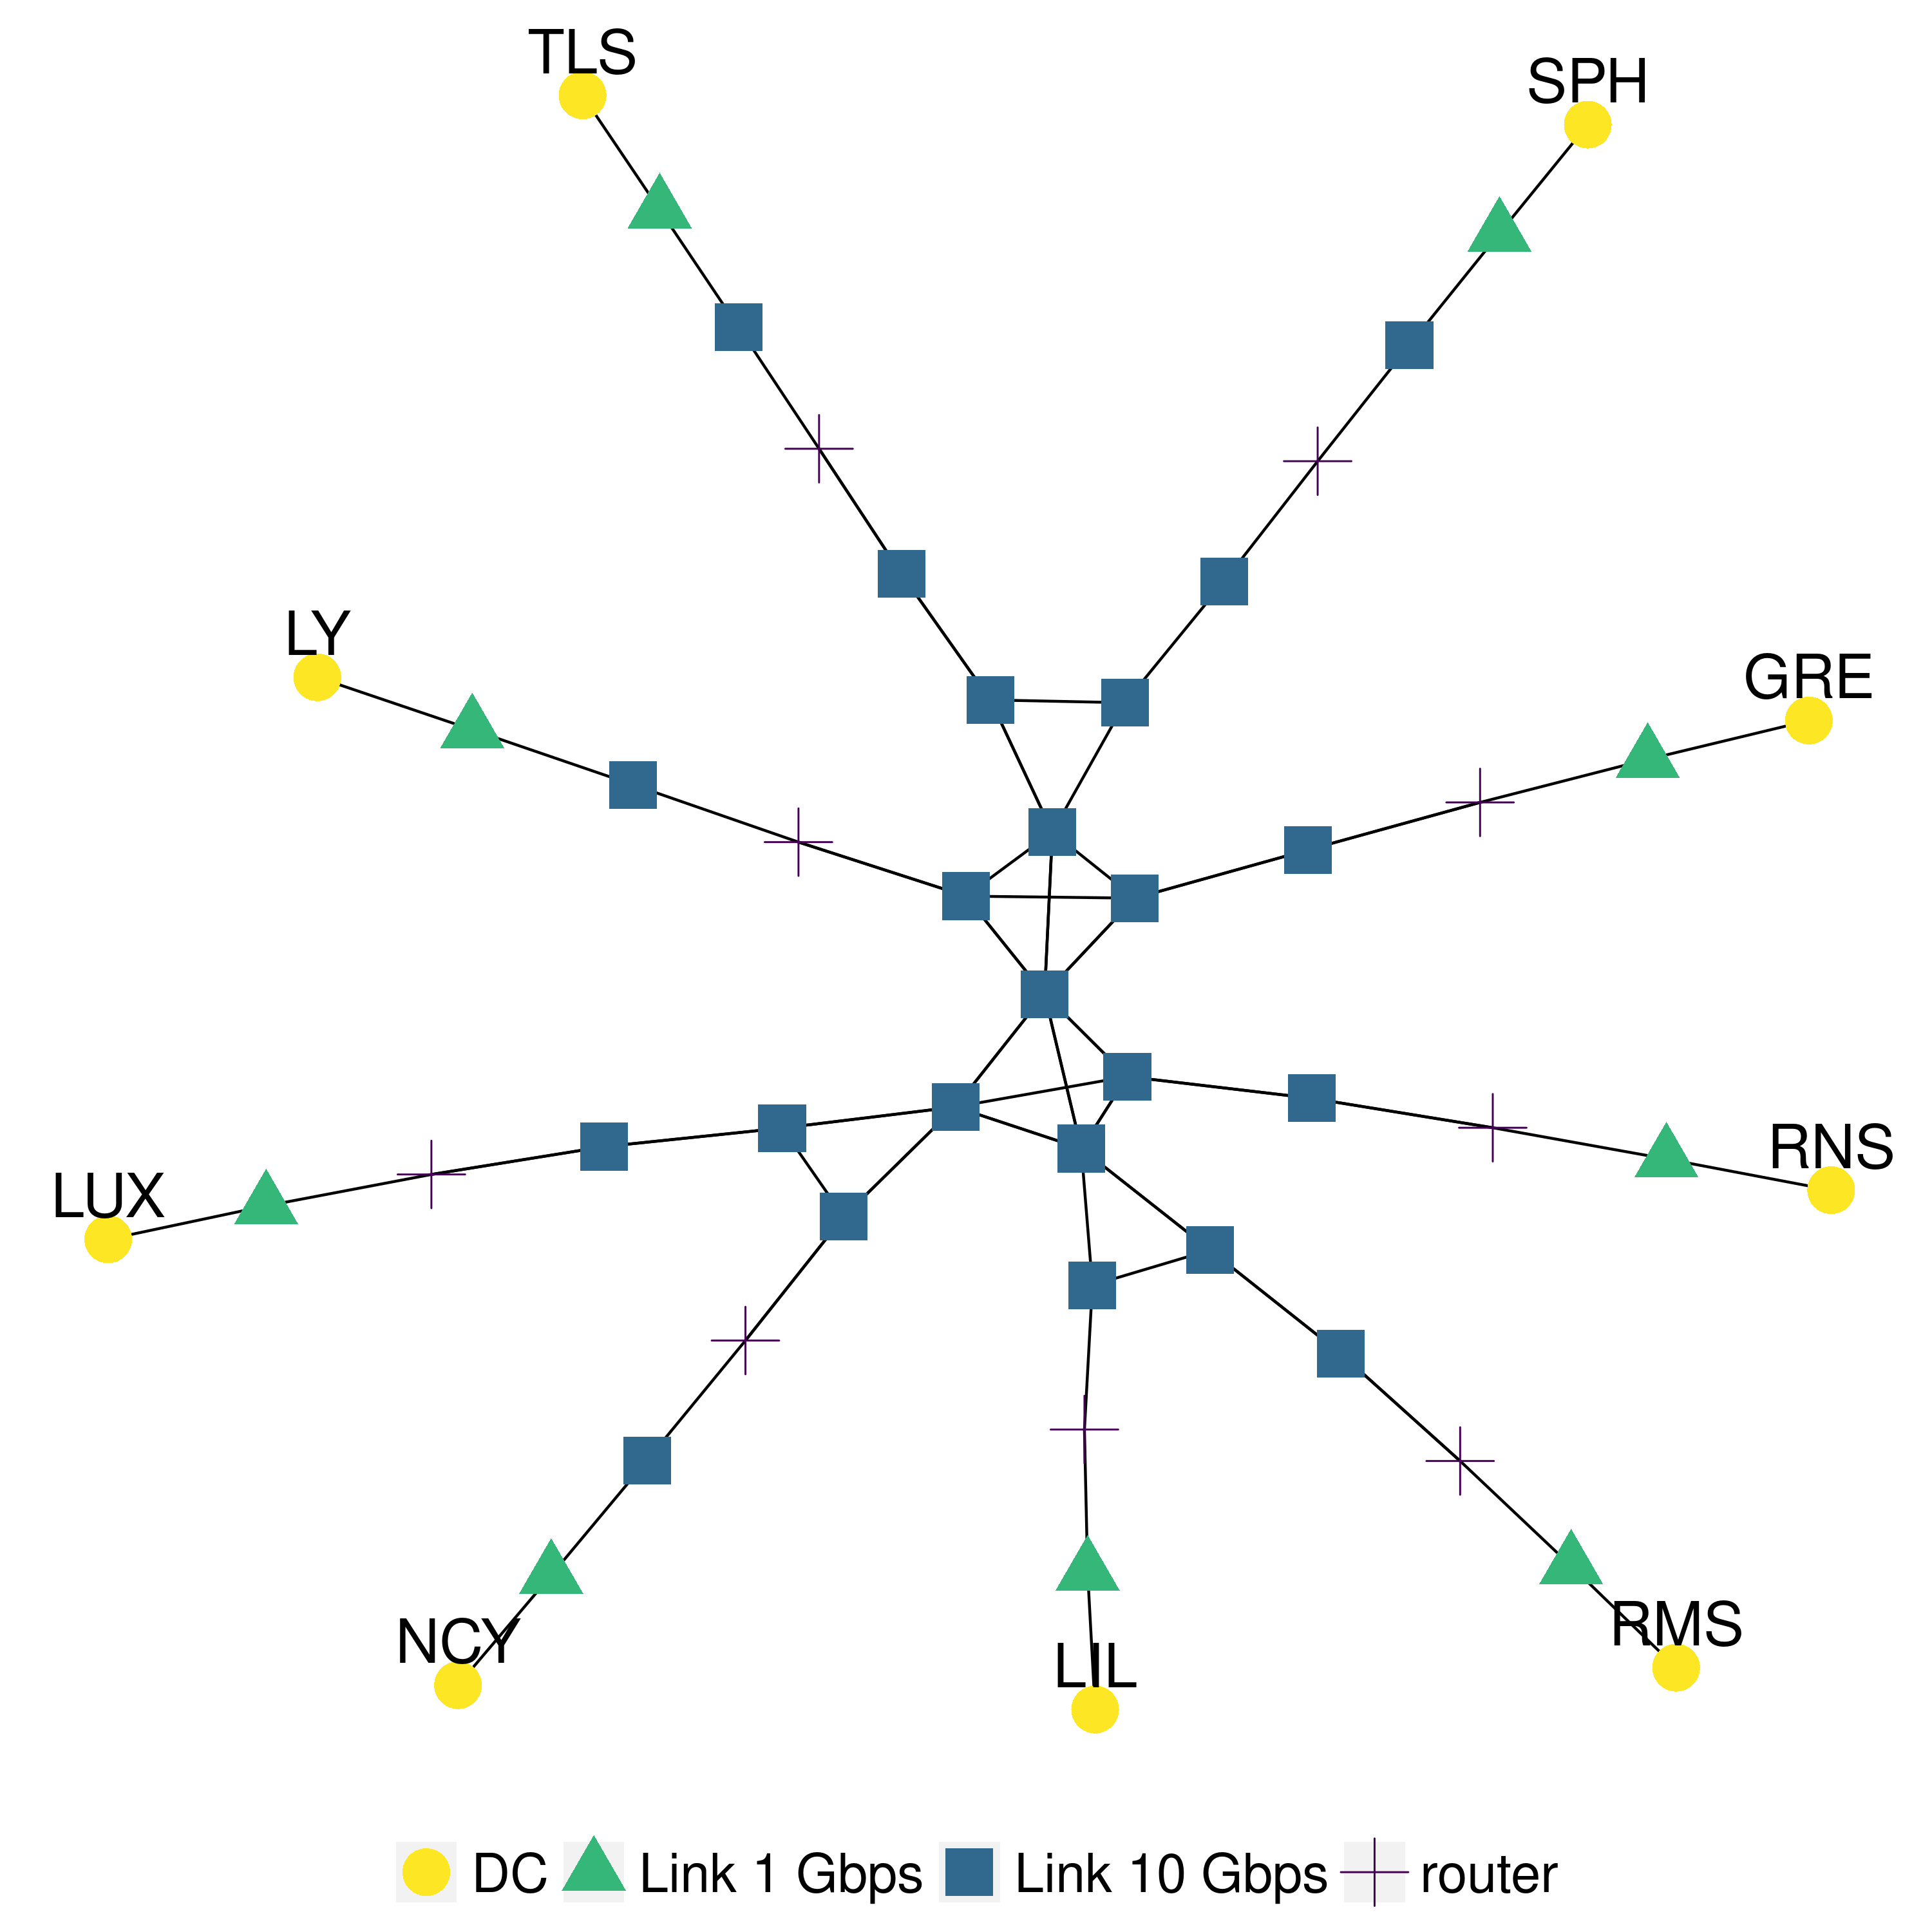
\includegraphics[width=\textwidth]{images/topology.png}
        \caption{DCs and how they are connected in the network.}
      \end{figure}
    \end{column}        
  \end{columns}    
\end{frame}


\begin{frame}{My research interests}

  Sizing the renewables infrastructures:
  
  \begin{itemize}
      
  \item Compute the area of solar panels (PVs) in m² and batteries capacity in Wh
  
  \end{itemize}

  Collaboration with researchers from the DATAZERO 2 project:
  Jean-Marc Nicod, Georges Da Costa, Veronika Rehn-Sonigo

\end{frame}



\begin{frame}{Sizing renewable infrastructures}  
  \textbf{Data centers:}
  
  \begin{itemize}

  \item Infrastructure already built (servers, network)
  \item Homogeneous (regarding CPU cores)
  \item Server power consumption: idle and dynamic 
  \item Intra network power consumption: static 
  \item Specific Power Usage Effectiveness (PUE) for each DC

  \end{itemize}

  \begin{figure}[!h]
    \centering
    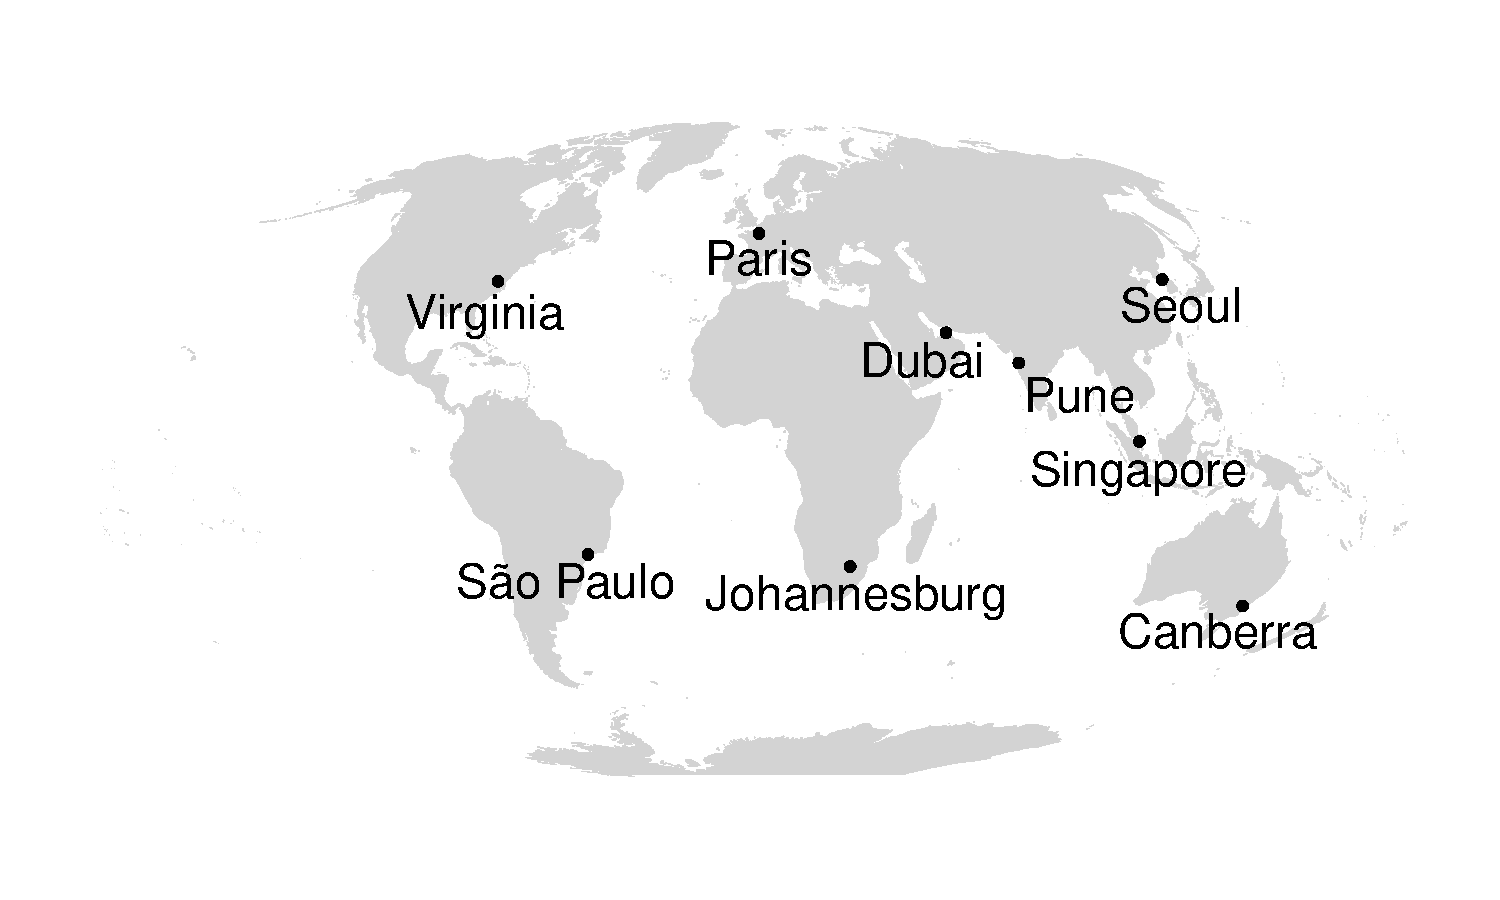
\includegraphics[width=0.6\textwidth]{images/locations_.pdf}
    \caption{Selected data centers location (inspired from Microsoft Azure)}
  \end{figure}  
\end{frame}

\begin{frame}{Sizing renewable infrastructures}  
  \textbf{Workload:}
  
  \begin{itemize}  
  \item All tasks must be scheduled and executed on time
  \item Batch tasks that can be executed in any of the DCs 
  \item No migration 
  \item Task execution cannot be delayed
  \end{itemize}

\end{frame}

\begin{frame}{Sizing renewable infrastructures}
  
  \textbf{Renewables infrastructure}
  
  \begin{itemize}    
  \item Batteries charge and discharge efficiency, Maximum Depth of Discharge
  \item PV panels efficiency    
  \item Carbon emissions from manufacturing (PV: 250 kg \ch{CO2} eq per m², bat: 59 kg \ch{CO2} eq per kWh)
  \item Lifetime (PV: 30 years, bat: 10 years)      
  \end{itemize}
  
\end{frame}

\begin{frame}{Sizing renewable infrastructures}
  
  \textbf{Local electricity grid}
  
  \begin{itemize}
    
  \item The energy mix is different at each location
  \item May have the presence of renewables or low carbon-intensive sources    
    
    \begin{table}
      
      \caption{Emissions (in g\ch{CO2}-eq/kWh) for using the regular grid. Source for grid emissions: electricityMap, climate-transparency.org.}\label{tab:carbonfootprint} \centering
      \footnotesize
      \begin{tabular}{|l|r|}
        
        \hline

        \textbf{Location} &  \textbf{Emissions }  \\
        \hline
        Johannesburg & 900.6  \\
        \hline
        Pune & 702.8\\
        \hline
        Canberra & 667.0 \\
        \hline
        Dubai & 530.0   \\
        \hline
        Singapore & 495.0  \\
        \hline     
        Seoul & 415.6  \\
        \hline
        Virginia  & 342.8  \\
        \hline
        São Paulo &  61.7 \\
        \hline 
        Paris &  52.6  \\
        \hline  

      \end{tabular}  
    \end{table}
    
  \end{itemize}
  \normalsize
\end{frame}


\begin{frame}{Proposed solution}
 
  Linear program formulation to minimize the carbon emissions from the cloud federation operation (timespan of 1 year) \footnotemark[2]
  
  \begin{itemize}
    
  \item Scheduling and dimensioning modeled as single problem
    \begin{itemize}
      
    \item Allocate workload to other DC or increase the battery capacity or PV area?
    \end{itemize}
    
  \item Only real variables 
    \begin{itemize}     
    \item  \alert{Optimal} solution in \alert{polynomial time}: 394264 variables, solved in less than \alert{1 minute} with Gurobi

    \end{itemize}

  \end{itemize}
  
  
  
  \footnotetext[2]{M. Vasconcelos, D. Cordeiro, G. Da Costa, F. Dufossé, J.-M. Nicod, and V. Rehn-Sonigo, ``Optimal sizing of a globally distributed low carbon cloud federation''. \textit{In: 2023 23nd IEEE International Symposium on Cluster, Cloud and Internet Computing (CCGrid), Bengaluru, India, 2023.}}
\end{frame}

\begin{frame}{  Linear Program summary}

  \alert{Obj. function:} Minimize the DC's operation \ch{CO2} emissions (1 year)
  \begin{itemize}
  \item \ch{CO2} comes from: grid power, manufacturing PV and batteries
  \end{itemize}
  
  \begin{columns}[T]
    \begin{column}{0.55\textwidth}
      \pause
      \alert{Input}

      \begin{itemize}
      \item Power consumption of servers and network equipment
      \item 1 year of workload  (Google trace)
      \item Renewable infrastructure specs (efficiency, manufacturing \ch{CO2})
      \item For each DC:
        \begin{itemize}
        \item Solar irradiation (1 year)
        \item \ch{CO2} from electricity grid
        \item PUE       
        \item CPU cores number
        \end{itemize}
      \end{itemize}
      
    \end{column}

    \begin{column}{0.45\textwidth}
      
      \pause          
      \alert{Output}
      
      \begin{itemize}          
      \item PVs area (m²)          
      \item Batteries capacity (kWh)                  
      \item Carbon emissions 
      \item Schedule of the workload         
      \end{itemize}
    \end{column}
  \end{columns}      
\end{frame}



\begin{frame}{Results}
  \begin{table}[!ht]
    \caption{Total emissions for the different scenarios.}\label{tab:emissions} \centering
    \begin{tabular}{|p{5cm}|r|}
      \hline
      \textbf{Scenarios} & \textbf{Emissions (t \ch{CO2}-eq)}   \\
      \hline
      Electrical grid                    & 201 211.3    \\
      \hline
      PV and batteries  &                  42 370.6 \\ 
      \hline
      PV, batteries, and grid            &  29 600.6   \\
      \hline
    \end{tabular}
  \end{table}

    Reductions on carbon emissions:
  
  \begin{itemize}
  \item Grid vs DC renewable infra : \alert{$\simeq 5$ times}
  \item Grid vs hybrid configuration (DC renewables and grid) : \alert{$\simeq 6$ times}
  \end{itemize}


  
\end{frame}





\begin{frame}{Results}
  \begin{figure}[!htbp]
    \centering
    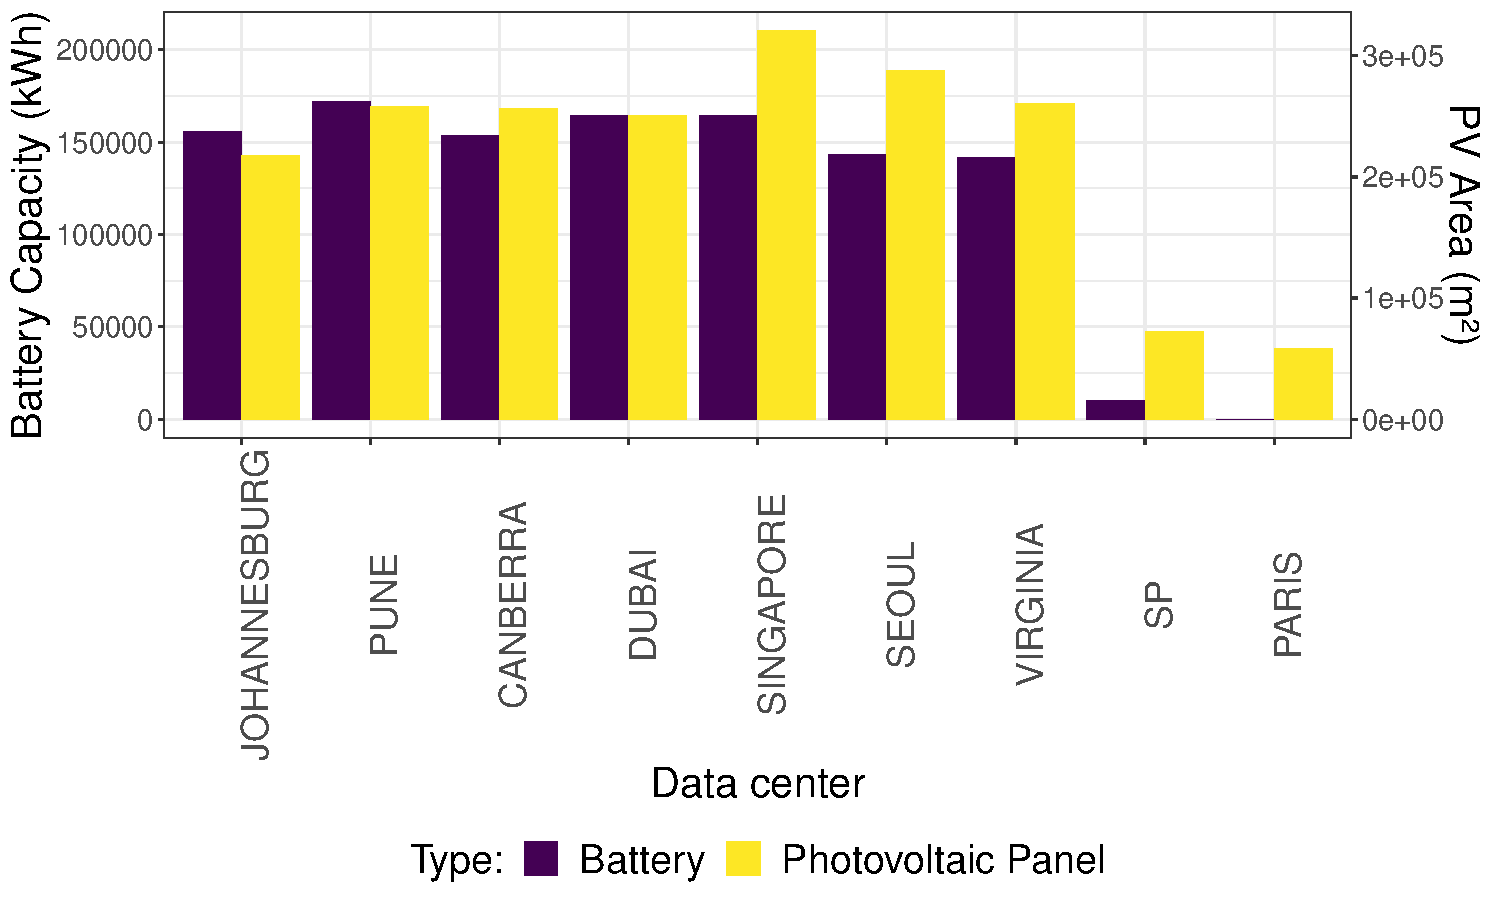
\includegraphics[width=1\textwidth]{images/sizing.pdf}
    \caption{Optimal result for the area of PV panels and capacity of the batteries.}
    \label{fig:sizing}
  \end{figure}
\end{frame}

\begin{frame}{Results}

  \begin{figure}[!htbp]
    \centering
    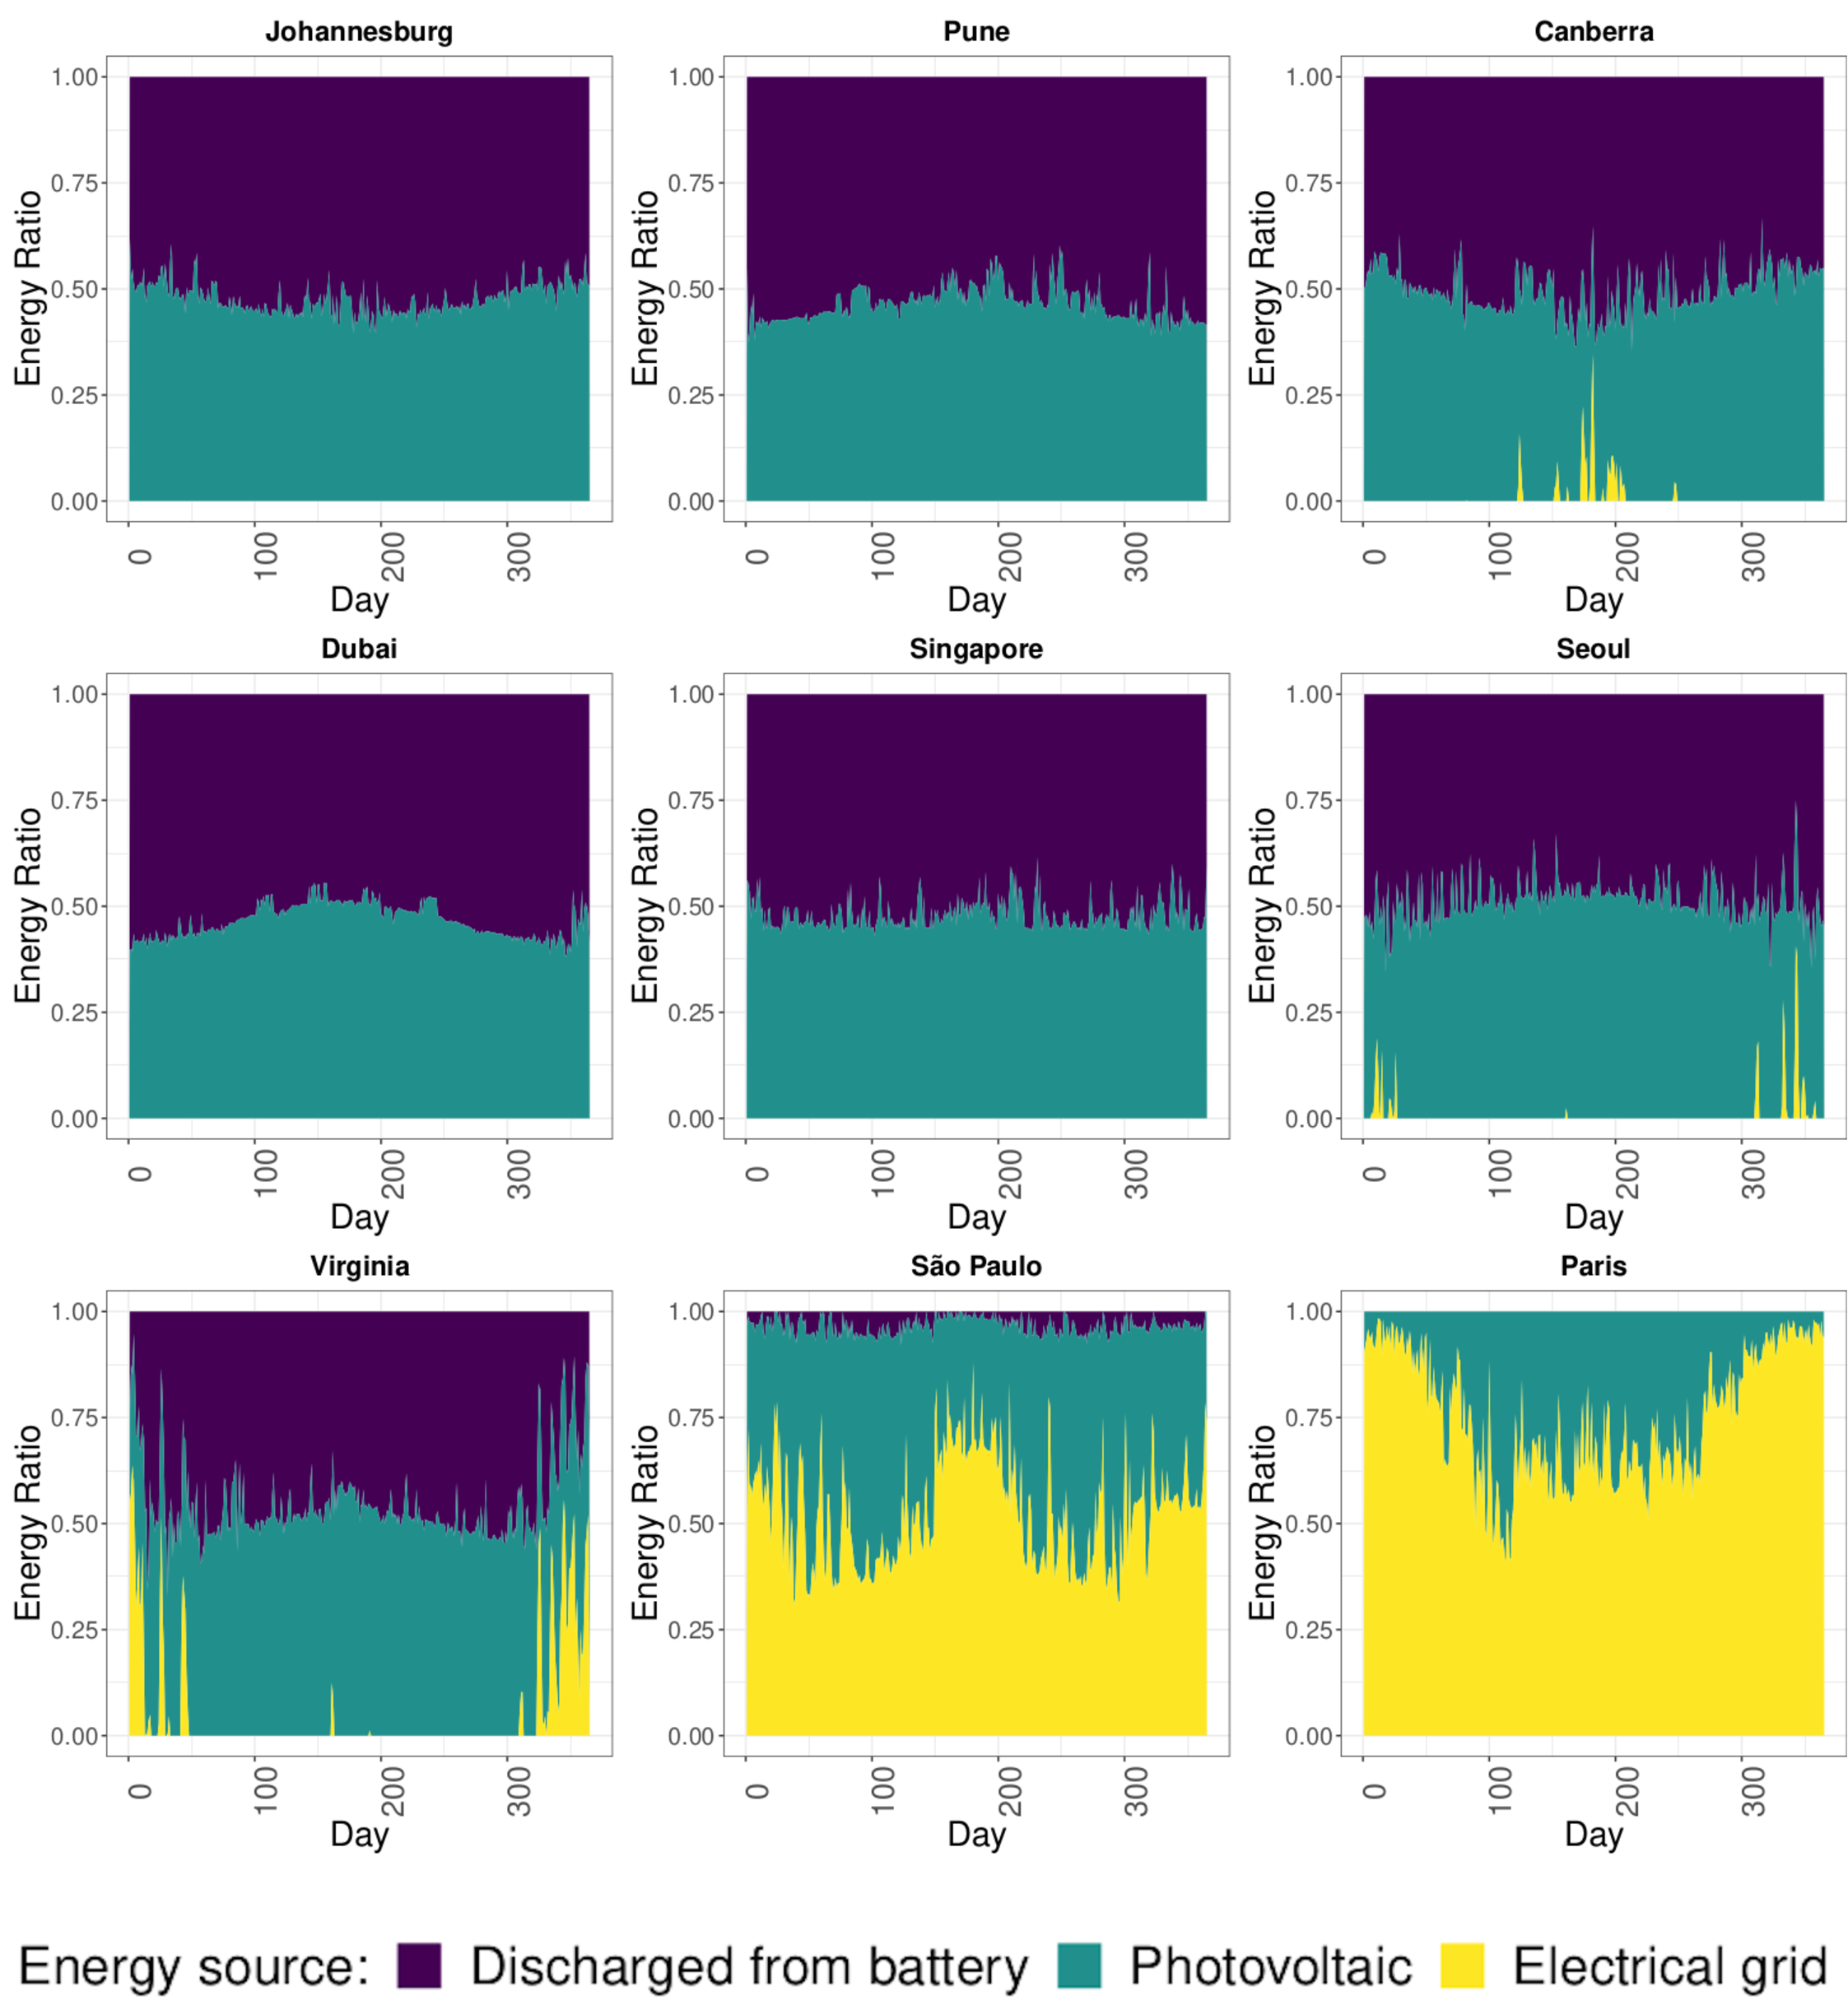
\includegraphics[width=.6\textwidth]{images/energy_ratio.pdf}
    \caption{Composition of the DCs’ daily energy consumption throughout the year considering the different sources of energy}
    \label{fig:sizing}
  \end{figure}

\end{frame}


\begin{frame}{Sizing for the long term:}

  Evaluate other strategies to further reduce the emissions  and for the long term:
  
  \begin{itemize}

  \item Consider the emissions from the life cycle
  \item How much including wind power could reduce the emissions?
  \item Impact of other scheduling algorithms in the total emissions (for example, allowing to delay some tasks)
  \item How expensive is it to reduce the carbon emissions of the cloud operation (monetary costs in dollars)
  \item Dimensioning of IT infrastructure (servers considering the footprint of manufacturing, new generations that are more  efficient)    

  \end{itemize}

  
\end{frame}


\begin{frame}{Impact of adding wind turbines (WT) }

  \begin{itemize}    
     \item  Can further reduce 34\% the carbon emissions in comparison
       to only using PVs and batteries.
     \item However, requires larger land area (1 to 3 WT per km²)
  \end{itemize}




  \begin{table}[h]
  \caption{Computed number of WT for each location.}\label{tab:results_wt} \centering
  \begin{tabular}{|l|r|}
  \hline
    
  \textbf{Location} &   \textbf{Number of WT} \\
  \hline
  Johannesburg & 59   \\
  \hline
  Pune         & 26 \\
  \hline
  Canberra    & 67 \\
  \hline
  Dubai       &  79  \\
  \hline
  Singapore   & 37 \\
  \hline     
  Seoul       & 109  \\
  \hline
  Virginia   & 39 \\
  \hline
  São Paulo   & 87 \\
  \hline 
  Paris    &   22 \\
  \hline
  
\end{tabular}  
\end{table}
  
\end{frame}



\begin{frame}{Impact of adding wind turbines (WT) }

  \begin{itemize}    
     \item  Can further reduce 34\% the carbon emissions in comparison
       to only using PVs and batteries.
     \item However, requires larger land area (1 to 3 WT per km²)
  \end{itemize}



\begin{table}[H]
  
  \caption{Capacity Factor (in \%) for solar panels and wind turbines at each location.}\label{tab:capacity_factor} \centering
  
  \begin{tabular}{|l|r|r|}
  \hline    
  \textbf{Location} &   \textbf{PV} & \textbf{WT}  \\
  \hline
  Johannesburg & 25.55 & 12.96  \\
  \hline
  Pune        &  24.26   & 10.04    \\
  \hline
  Canberra    & 22.08    & 12.97  \\
  \hline
  Dubai      & 25.28      & 13.98   \\
  \hline
  Singapore & 17.68    & 8.58   \\
  \hline     
  Seoul      & 18.81   &  9.41   \\
  \hline
  Virginia   & 19.83   &  14.68 \\
  \hline
  São Paulo  & 21.74   &  10.06    \\
  \hline 
  Paris      & 15.37   &  23.51   \\
  \hline  

\end{tabular}
\end{table}
  
\end{frame}




\begin{frame}{Flexibility in the scheduling}
  
  What is the impact in carbon emissions of delaying $\alpha$ percent of the jobs up to $\beta$ time slots (1h per time slot) ?
  \pause

  \begin{table}[h]
\caption{Reductions in total carbon emissions ( \% ) in comparison to the scenario where it is not possible to delay the workload. }\centering
\label{tab:flex_scheduling}
\begin{tabular}{|l|r|r|r|r|r|r|r|r|r|}
  \hline
  \small
\backslashbox{$\alpha$}{$\beta$} &   \textcolor{black}{\textbf{ 1}} &  \textcolor{black}{\textbf{ 24 }} &  \textcolor{black}{\textbf{ 48 }}  &   \textcolor{black}{\textbf{ 72 }} &   \textcolor{black}{\textbf{ 96 }} &   \textcolor{black}{\textbf{ 120  }} &   \textcolor{black}{\textbf{ 144 }} &   \textcolor{black}{\textbf{ 168 }} \\ 
     \hline
 \textcolor{black}{ \textbf{10}}   &  0.46  &  3.14 &  3.48 &  3.66 &  3.76 &  3.81 &  3.85 &  3.85 \\ 
\hline
 \textcolor{black}{ \textbf{20}}   &  0.84  &  3.85 &  4.11 &  4.21 &  4.21 &  4.21 &  4.22 &  4.22 \\ 
\hline
 \textcolor{black}{ \textbf{30}}   &  1.15  &  4.07 &  4.25 &  4.25 &  4.26 &  4.26 &  4.27 &  4.27 \\ 
\hline
 \textcolor{black}{ \textbf{40}}   &  1.42  &  4.15 &  4.25 &  4.26 &  4.27 &  4.28 &  4.28 &  4.29 \\ 
\hline
 \textcolor{black}{ \textbf{50}}   &  1.65  &  4.22 &  4.26 &  4.27 &  4.28 &  4.29 &  4.3 &  4.3 \\ 
\hline
\end{tabular}
\end{table}

\end{frame}

\begin{frame}{Costs (\$) of reducing the environmental impact}

  \begin{itemize}

  \item   Considered the Levelized Cost of Energy
  \item Grid price is half at off-peak times (10 pm to 8 am)
  \item   Battery price: 0.20 dolars per kWh of electricity delivered

  \end{itemize}
 
 \begin{table}
   
  \caption{Price of different sources of energy (USD per kWh) at each location.  }\label{tab:price_electricity_sources} \centering
  \small
  \begin{tabular}{|l|r|r|r|}
  \hline    
  \textbf{Location} &   \textbf{Grid} & \textbf{PV} & \textbf{WT} \\
  \hline
  Johannesburg & 0.074 & 0.0385  &  0.1984           \\
  \hline 
  Pune         &  0.104   & 0.0406  & 0.2610         \\
  \hline 
  Canberra     & 0.331    &  0.0445 & 0.1993         \\
  \hline
  Dubai        & 0.101      & 0.0390  &   0.1863     \\
  \hline
  Singapore    & 0.272    & 0.0557  & 0.3009         \\
  \hline     
  Seoul        & 0.092   & 0.0525  & 0.2735          \\
  \hline
  Virginia     & 0.150   &  0.0498 &  0.1760         \\
  \hline
  São Paulo    & 0.144   &  0.0453 & 0.2572          \\
  \hline 
  Paris        & 0.340   &  0.0643 & 0.1098          \\
  \hline
\end{tabular}
\end{table}

\end{frame}



\begin{frame}{Costs (\$) of reducing the environmental impact}


\begin{table}[h]
  \caption{Total costs (millions of \$) and carbon emissions ($t\,\ch{CO2}\text{-}eq$) for the different scenarios. }\label{tab:total_price_and_co2_grid_timeseries} \centering
  \begin{tabular}{|l|r|r|}
   \hline  
  \textbf{Scenario} &   \textbf{ Millions of \$}  &  \textbf{ $\mathbf{t\,\ch{CO2}\text{-}eq}$}  \\    
  \hline
  Min. cost (PV + WT + Bat + grid) & 36.7   & 141 001.67     \\
  \hline
  Min. cost (PV + Bat + grid)      & 38.3   & 145 193.64  \\
  \hline
  Min. cost (WT + Bat + grid)      & 51.1   &  204 568.07 \\
  \hline
  Min. \ch{CO2} (PV + Bat + grid) & 72.8     & 37 828.49        \\
  \hline
  Min. \ch{CO2} (WT + Bat + grid) & 277.5    &  58 263.38  \\
  \hline
  Min. \ch{CO2} (PV +WT+  Bat + grid) & 117.3 &  24 977.89  \\
  \hline
  Only grid                           & 56.7        & 222 876.62       \\
  \hline
  \end{tabular}  
\end{table}

\end{frame}


\begin{frame}{Sizing the IT part}
  
  \begin{itemize}
  \item Workload growth over time
   \item New hardware generations that may be more power-efficient
    \item \ch{CO2} from manufacturing the servers      
  \end{itemize}

\end{frame}


\begin{frame}{Sizing the IT part}


\textbf{Scenarios:}
\begin{itemize}
  \item Use the current infrastructure at maximum, and only buy new servers to meet the workload demand   
  \item Can manufacture and replace old servers to minimize the total carbon emissions    
\end{itemize}

\textbf{Settings:}

\begin{table}[h]
  \small
  \caption{Servers specifications for different generations.} \centering
  \label{tab:servers_specs} 
  \begin{tabular}{|l|r|r|r|r|r|}
  \hline    
  \textbf{Year} & \textbf{CPU} &   \textbf{Cores} & \textbf{Pidle}  & \textbf{Pcore}  & \textbf{$\mathbf{kg\,\ch{CO2}\text{-}eq}$}  \\
  \hline
  < 2016      & Intel Xeon E5-2660 v2 & 20 & 52 & 7.5  & -   \\
  \hline
  2017 & Intel Xeon Platinum 8180 & 56 & 48.9 & 6.68  & 578.6   \\
  \hline
%  2019, 2020   & AMD EPYC 7742  & 64 & 66.1 & 2.71  & 587.2 \\
 % \hline
  %2021        & AMD EPYC 7763 & 128 & 75.6 & 3     & 590.3 \\
  %\hline
\end{tabular}  
\end{table}



 \begin{itemize}
  \item Workload 22\% increase per year (CISCO)
  \item Server life time of 4 years
  \end{itemize}

\end{frame}



\begin{frame}{Sizing the IT part}
  

\textbf{Scenarios:}
\begin{enumerate}
  \item Use the current infrastructure at maximum, and only buy new servers to meet the workload demand   
  \item Can manufacture and replace old servers to minimize the total carbon emissions    
\end{enumerate}

\textbf{Results:}
\begin{itemize}
  \item Scenario 2 had a 10\% lower carbon footprint, and manufactured
    8\% more servers.
\end{itemize}
  
\end{frame}

\begin{frame}{Sizing the IT part}
  
  \begin{center}
    \begin{figure}[h]
      \centering
      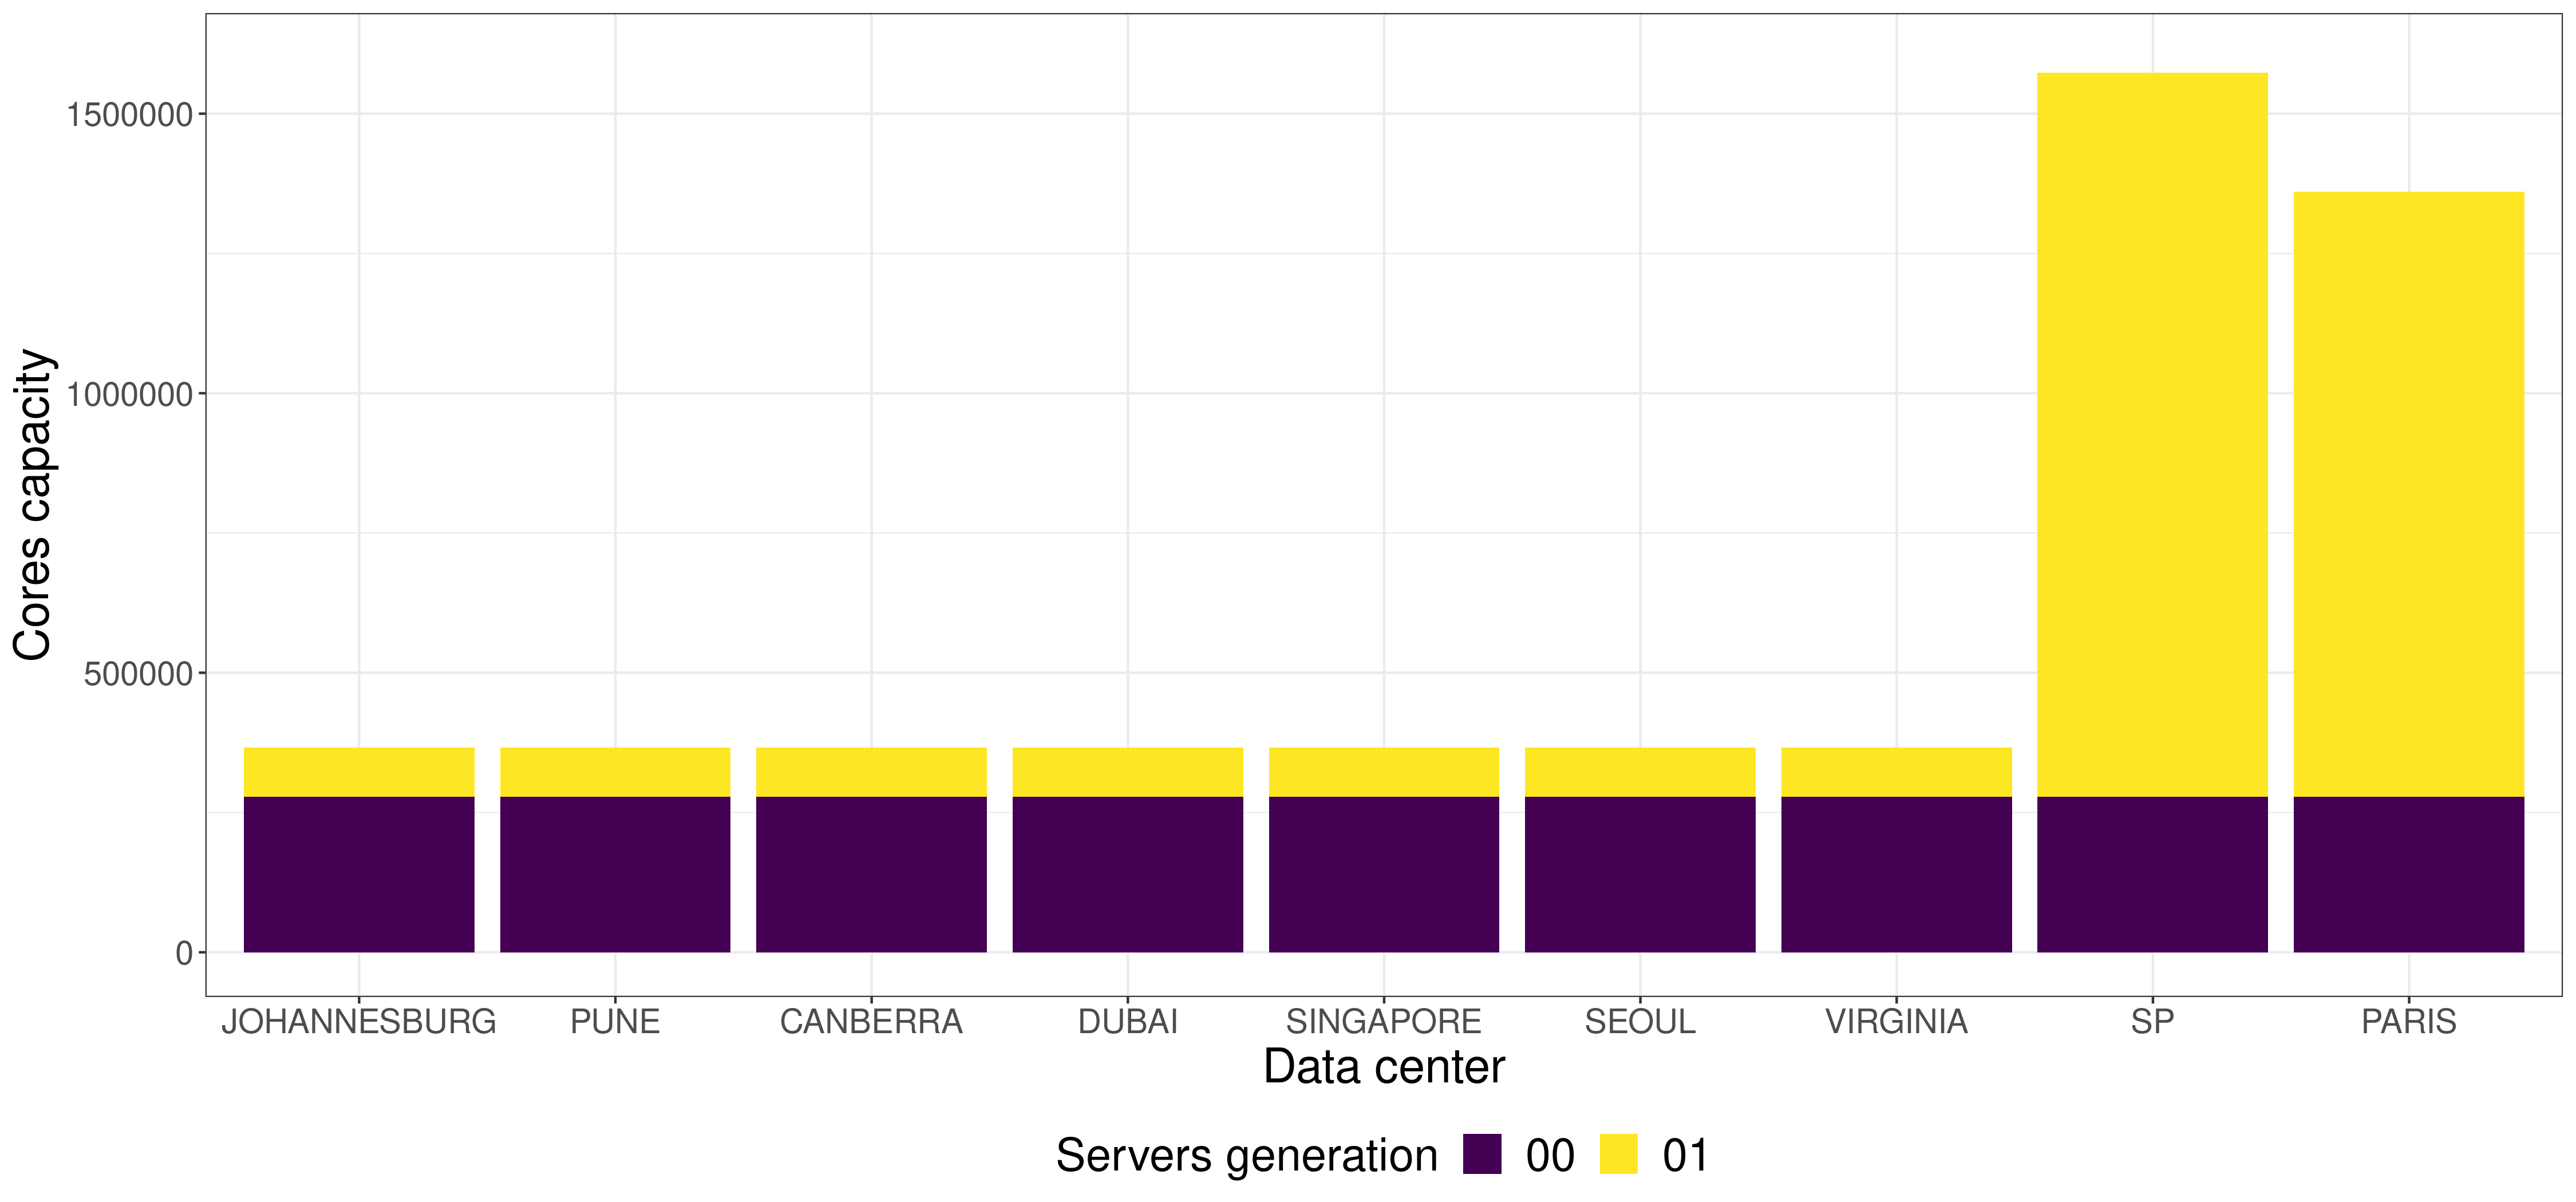
\includegraphics[width=\textwidth]{images/cloud_federation_only_add.png}
      \caption{Sizing for the scenario 1 - Only add new servers.}
    \end{figure}
  \end{center}


\end{frame}
\begin{frame}{Sizing the IT part}
  

  \begin{center}
    \begin{figure}[h]
      \centering
      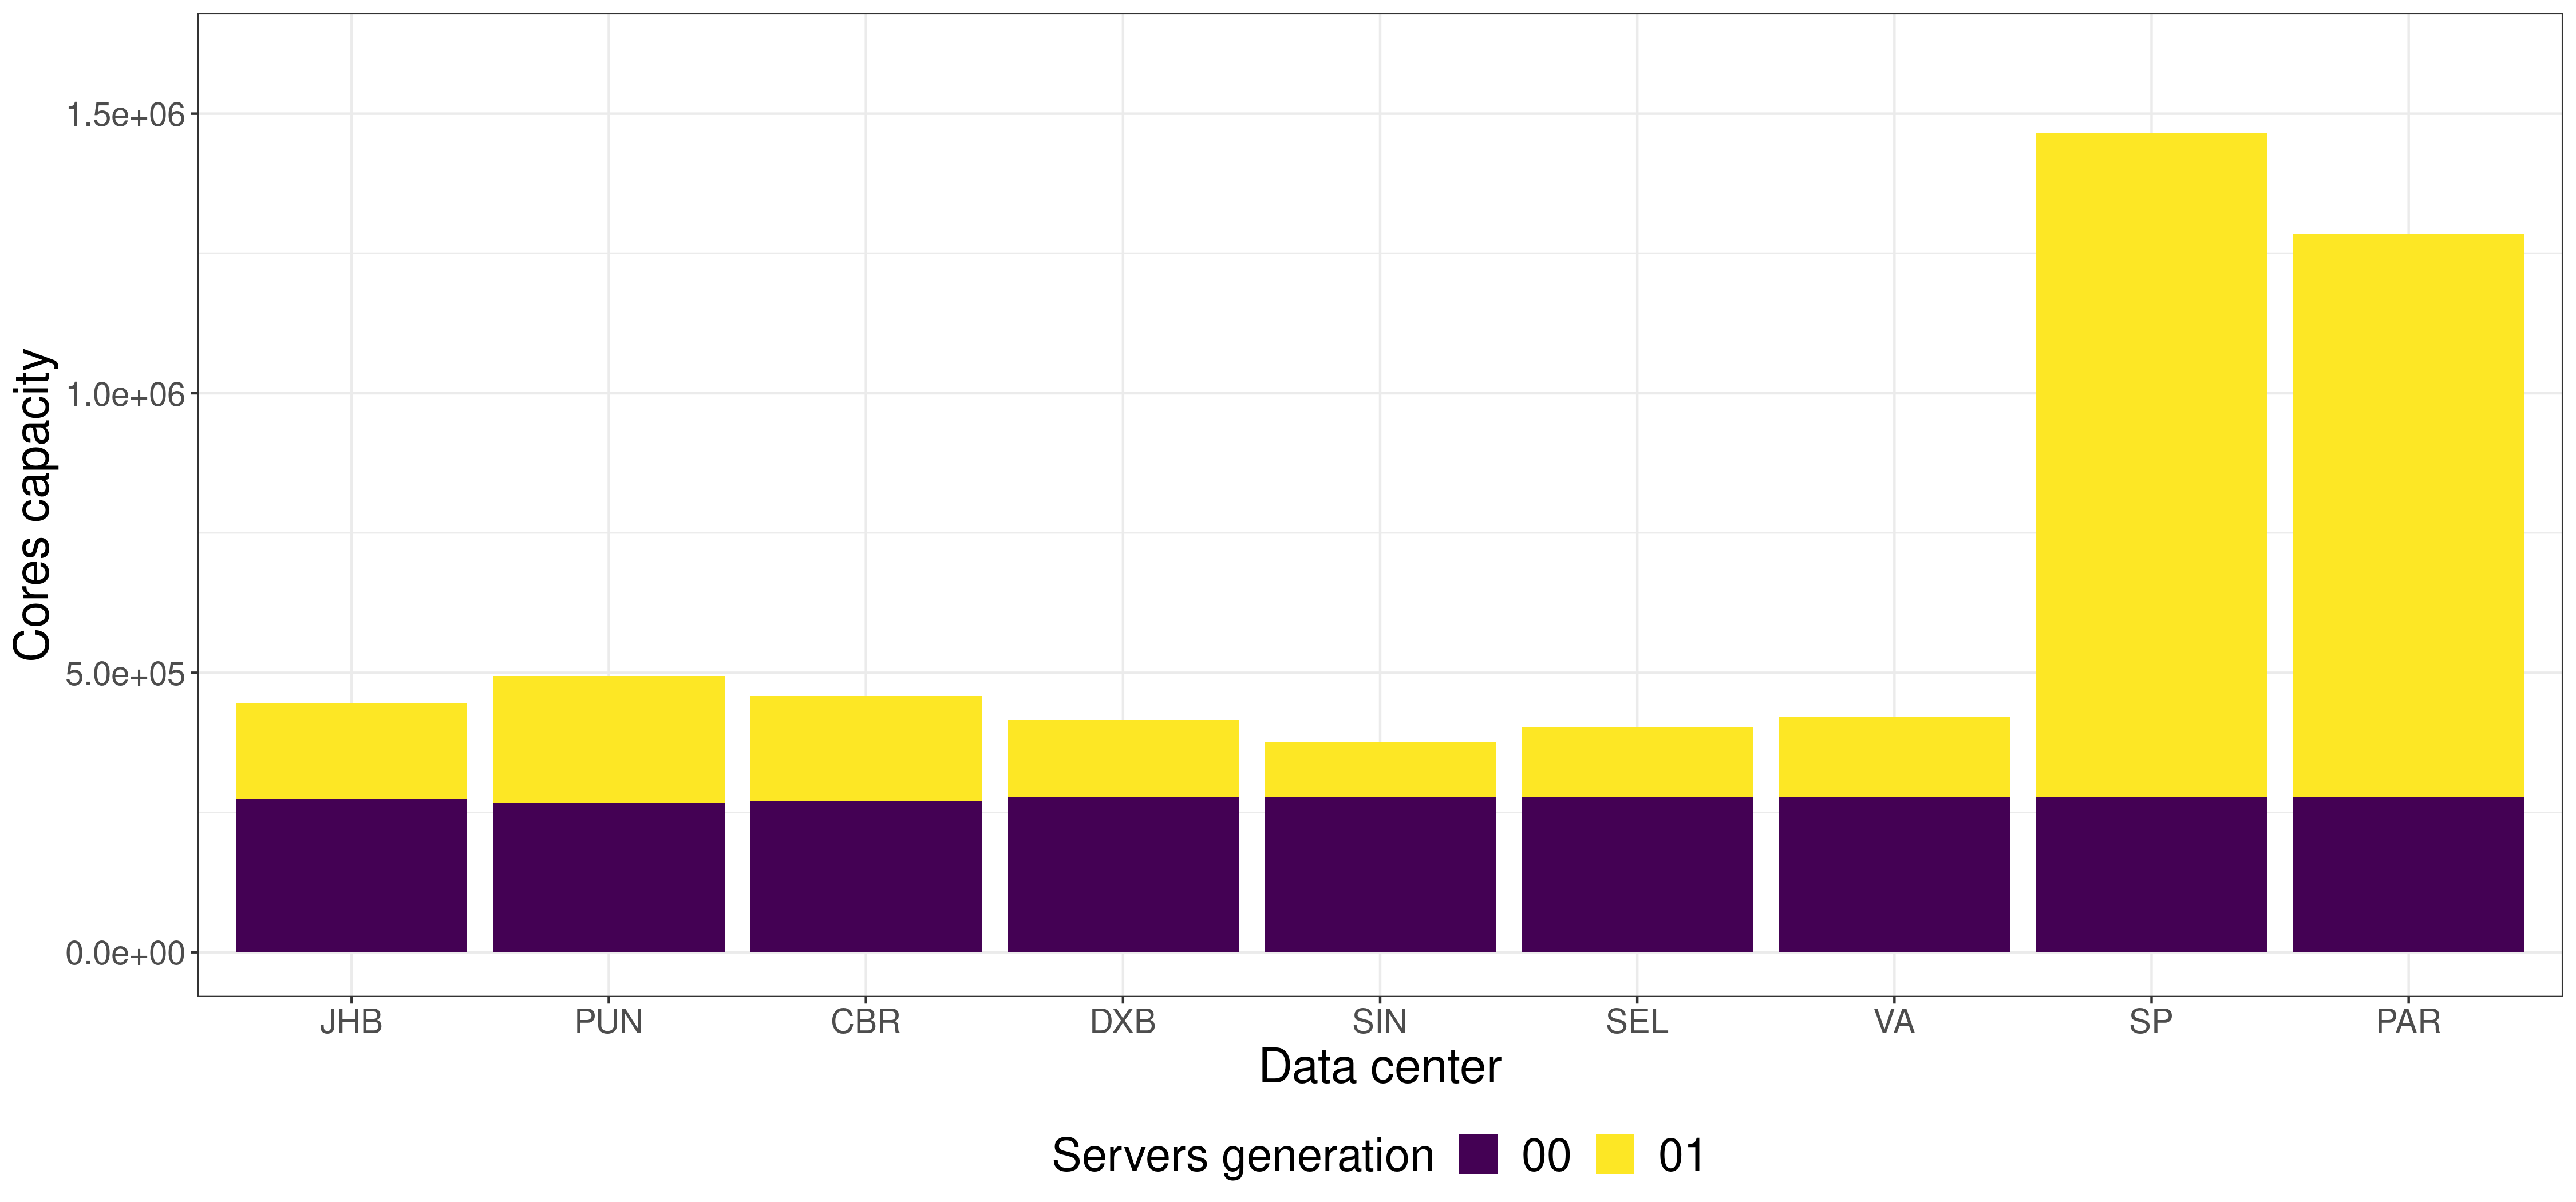
\includegraphics[width=\textwidth]{images/cloud_federation_add_replace.png}
      \caption{Sizing for the scenario 2 - Add new servers and replace old ones.}
    \end{figure}
  \end{center}


\end{frame}





\begin{frame}{Sizing the IT part}


\textbf{Scenarios:}
\begin{itemize}
 \item Decision made year by year (greedy approach)
 \item Optimal solution (all info is know in advance)
\end{itemize}

\textbf{Settings:}

\begin{table}[h]
  \small
  \caption{Servers specifications for different generations.} \centering
  \label{tab:servers_specs} 
  \begin{tabular}{|l|r|r|r|r|r|}
  \hline    
  \textbf{Year} & \textbf{CPU} &   \textbf{Cores} & \textbf{Pidle}  & \textbf{Pcore}  & \textbf{$\mathbf{kg\,\ch{CO2}\text{-}eq}$}  \\
  \hline
  < 2016      & Intel Xeon E5-2660 v2 & 20 & 52 & 7.5  & -   \\
  \hline
  2017, 2018 & Intel Xeon Platinum 8180 & 56 & 48.9 & 6.68  & 578.6   \\
  \hline
  2019, 2020   & AMD EPYC 7742  & 64 & 66.1 & 2.71  & 587.2 \\
  \hline
  2021        & AMD EPYC 7763 & 128 & 75.6 & 3     & 590.3 \\
  \hline
\end{tabular}  
\end{table}

\end{frame}

\begin{frame}{Sizing the IT part}

  The optimal solution emits 13.4\% less \ch{CO2}.

  \begin{center}
    \begin{figure}[h]
      \centering
      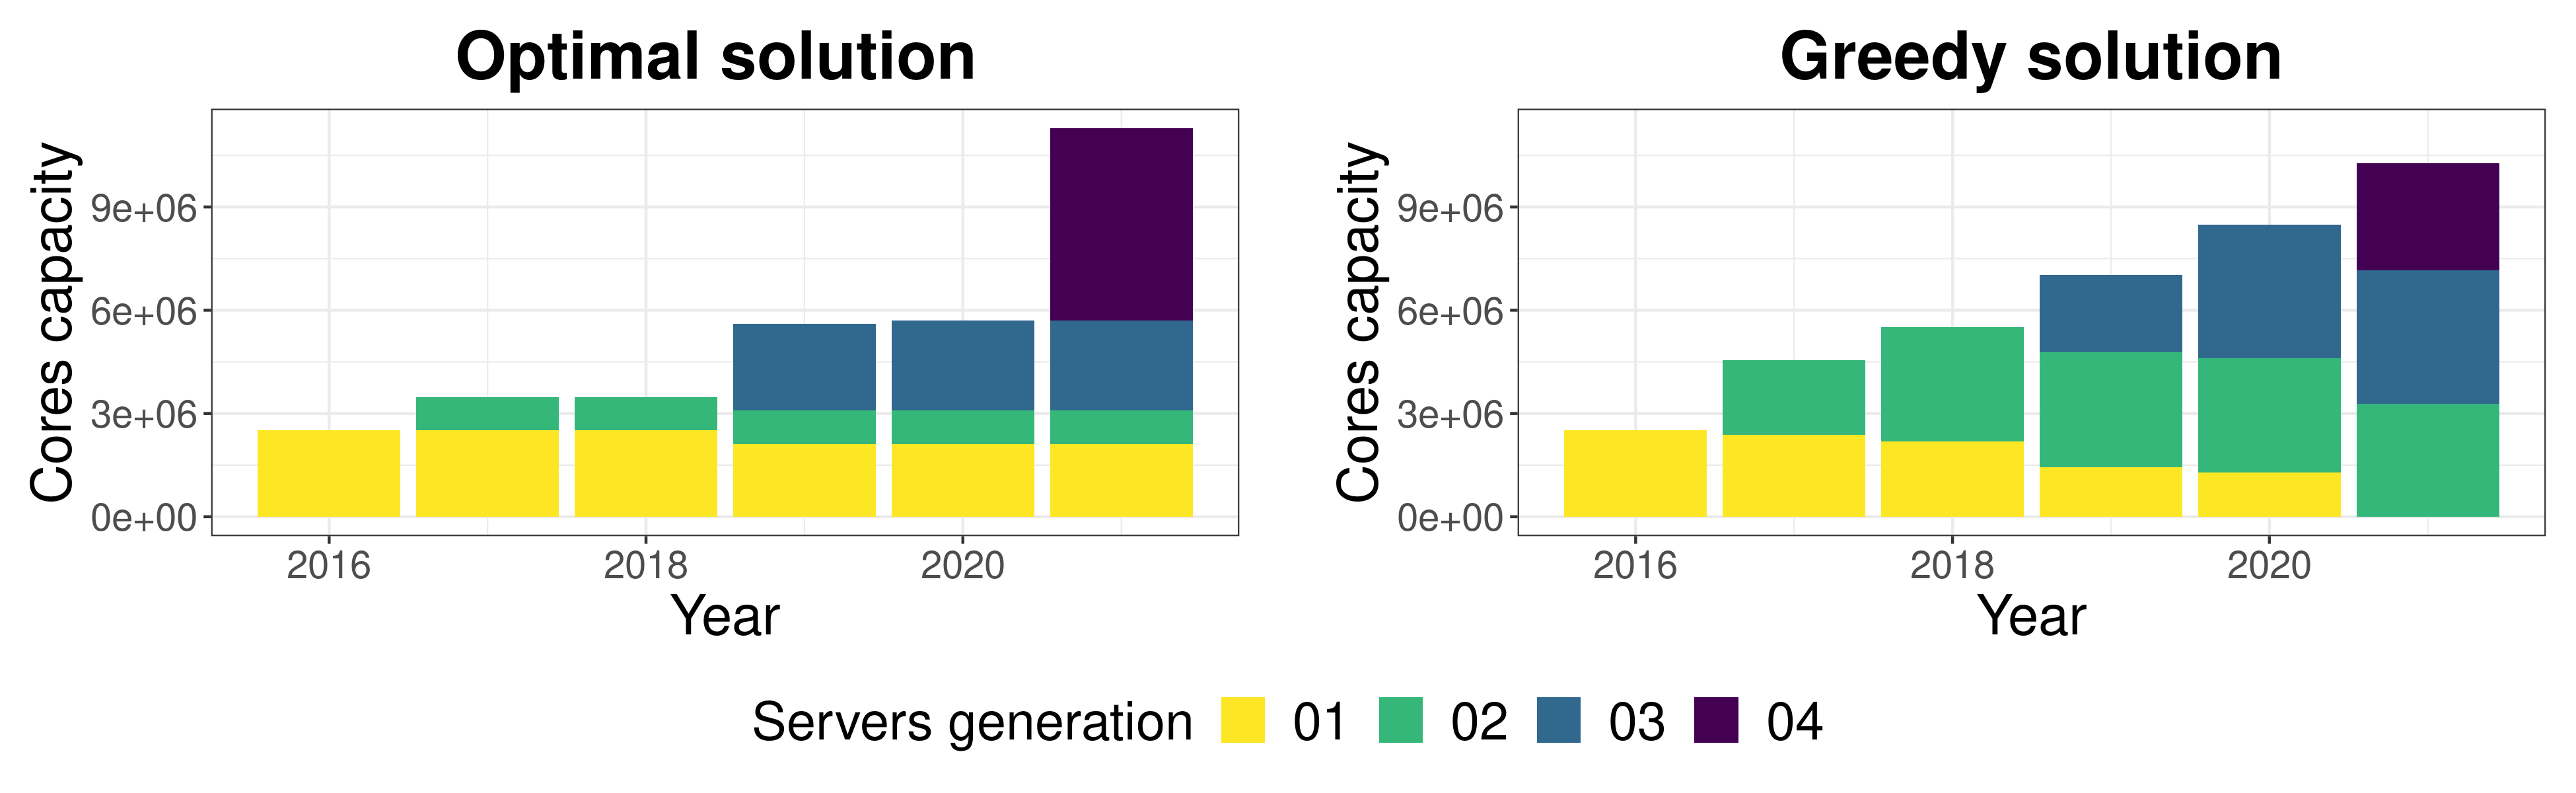
\includegraphics[width=.77\textwidth]{images/cloud_federation_evolution_lifetime.png}
      \caption{Comparison between the optimal and greedy approaches.}
    \end{figure}
  \end{center}


\end{frame}


\begin{frame}{Future work}


  \begin{itemize}
   
  \item What could be learned from the optimal solution of adding/replacing servers ?
  \item Costs of the servers     
  \item Degradation of the renewable infrastructure over the years
  \item Sizing new data centers ( renewable and IT infrastructure)
  \item Other types of environmental impact
    
  \end{itemize}    
\end{frame}


\begin{frame}[allowframebreaks]  
  \printbibliography
\end{frame}

\appendix

\begin{frame}{LP Overview}

  \alert{ Data center power consumption:}
  
  \begin{equation}
    P^d_k \leq Pre^d_k + Pgrid^d_k + Pdch_k^d - Pch_k^d   
  \end{equation}


  where $Pch_k^d$ is the power to charge the battery at each time of time slot $k$ on $DC^d$ and $Pdch_k^d$ is the power to discharge the battery, $Pre^d_k $ is the solar power produced, and $ Pgrid^d_k $ is the power used from the local grid.

  \alert{Workload:}
  
  \begin{equation} \label{eq:wk}
    w_k^d \leq C^d
  \end{equation}
  
  where $w_k^d$ is number of cores needed during the $k$th time slot on $DC^d$,  and  $C^d$ is the number of cores within $DC^d$ .
  
\end{frame}

\begin{frame}{LP Overview}

  \alert{Batteries level of energy ($B^d_ k$):} 

  \begin{equation} \label{eq:bdk}
    B^d_k = B^d_{k-1}  + Pch^d_{k-1} \times \eta_{ch} \times \Delta{t} - \frac{Pdch^d_{k-1}}{\eta_{dch}} \times \Delta{t}
  \end{equation}

  where $\eta_{ch}$ is efficiency of the charge process and $\eta_{dch}$ is the efficiency of the discharge process.

  \alert{Solar power production:}

  \begin{equation} \label{eq:predk}
    Pre^d_{k}= I^d_k \times Apv^d \times \eta_{pv}
  \end{equation}

  where $I^d_k$ is the solar irradiance, $Apv^d$ the PV panel area,  and $\eta_{pv}$ is the efficiency of PV module

\end{frame}


\begin{frame}{LP Overview}


  \alert{Objective function:}
  
  \begin{equation} \label{eq:FPALL}
    \text{minimize }\sum_{k=0}^{K-1} \sum_{d=1}^D ( FPgrid^d_k +  FPpv^d_k) + \sum_{d=1}^D FPbat^d
  \end{equation}

\end{frame}




\end{document}


Optimal sizing ...

1h

5 min

time slots..

recycling ...


migrate a real virutal machine


projects

ANR ....



https://facto.irisa.fr

power consumption of wifi chips
internet boxes ...


A terceira, como trabalhar nas camadas clouds ???


deploy openstack nas clouds ...


openstack ->>



tentar o openstack ...

mandar msgs pro george, pro laurent e pro romain r
